Third order Ambisonics encoder, B-format (FuMa channel
sequence ``wyzxvtrsuqomklnp'' and normalization).

\begin{lstlisting}[numbers=none]
<receiver type="amb3h3v"/>
\end{lstlisting}

$N=16$

To play back the content of a virtual scene on an arbitrary playback
device, we have to use an external tool to decode the ambisonics
format (a tool which will mix the ambisonics channels signals in an
appropriate way in order to get the signals for channels of our
playback system).  To achieve this, we can make a jack connection
between the output of the ambisonics receiver
(\verb!<scenename>.render:<receivername>.<channel>!) and ambisonics
decoder "ambdec"\index{ambdec}\index{decoder}:
%
\itscexamplepriv[linerange={2-5},numbers=none]{objects}
%
If we use connect="ambdec:in", then the connections will be done, so
that the channels have the same name in both receiver output and
ambdec input, as shown in the Figure \ref{fig:ambdec}. 
%
We can then go to the settings of the ambdec device and find a type of
output corresponding to our playback set up
(Config$>>$Load$>>$usr/share/ambdec/presets). 
%
For example if we choose a preset \textit{octagon-3h0v}, the
appropriate output ports will appear (Figure \ref{fig:ambdec_out}),
which can be then connected with the system playback devices.

\begin{figure}[htb]
  \centering
  \fbox{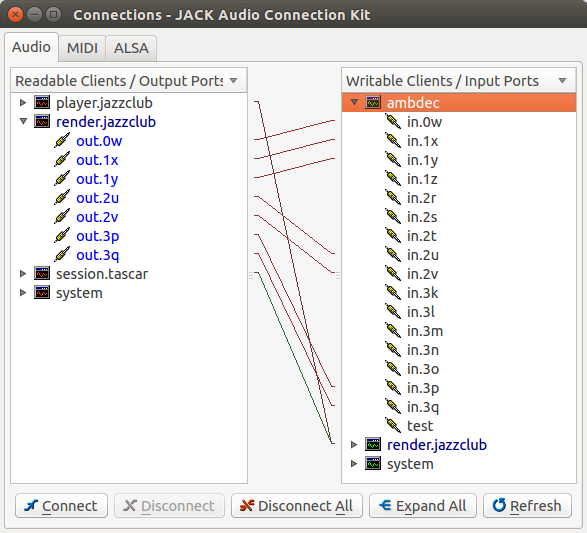
\includegraphics[width=0.8\textwidth]{render_ambdec.png}}
  \caption{Connections, which are created, when using attribute \attr{connect} in the element \elem{sound}}
  \label{fig:ambdec}
\end{figure}
 
 \begin{figure}[htb]
  \centering
  \fbox{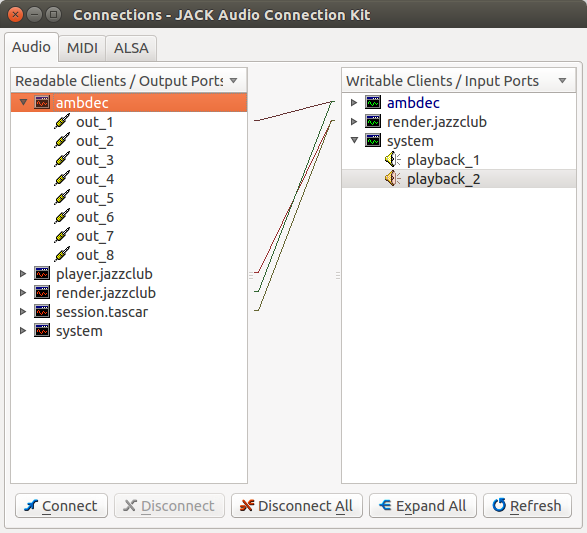
\includegraphics[width=0.8\textwidth]{ambdec_out.png}}
  \caption{Ambdec output ports for a horizontal octagon}
  \label{fig:ambdec_out}
\end{figure}
